\chapter{Implementation}
\section{Experimental Setup}
In order to conduct the training process described in the previous chapter, it was necessary to have a computer with a powerful GPU in order to speed up training. For this Master thesis, the training was conducted on a Nvidia Titan X (Pascal) GPU with 12 GB of memory. 
\newline\newline
For the ease of reproducibility of this work, frameworks and major libraries are hightlighted as follows: For machine learning, Keras 2.2.5 with TensorFlow 1.14.0 as a backend. In addition to that, Keras-VggFace 0.6, MTCNN 0.1.0 and OpenCV 4.1 were used. The entire code was implemented in a Python 3.6 environment.


\section{Dataset}
The selected Acted Facial Expressions in the wild - Valence Arousal (AFEW-VA) dataset introduced by \citet{Kossaifi:2017:AFEW-VADatabase} is based upon the Acted Facial Expressions in the wild database (AFEW) introduced in \citeyear{Dhall:2012:AFEW} by \citet{Dhall:2012:AFEW}. The AFEW dataset is composed of video clips that try to depict a real-world environment. It captures facial expressions, natural head pose movements, occlusions, subjects' races, gender, diverse ages, and multiple subjects in a scene. The authors labeled the video clips with one of six basic expressions: anger, disgust, fear, happiness, sadness, surprise, or neutral. The AFEW-VA dataset \citep{Kossaifi:2017:AFEW-VADatabase} uses the same underlying real-world video data, but did not annotate its video clips with one of six basic expressions. Instead it used the two dimensional affective space with valence and arousal. 
\newline\newline
Furthermore, as the name of the dataset already suggests, the dataset is compopsed of data that was collected under in-the-wild conditions. In-the-wild refers to real-life conditions in video clips, which make it significantly more challenging to recognize emotions in comparison to a dataset that has been captured in a controlled environment. \citet{Salah:2018:VideoBasedER} explained that these difficulties can be caused by, for example, uncontrolled illumination or uncontrolled video quality due to a different recording medium, like webcams by individuals vs. professional cameras. Such in-the-wild data is usually acquired from talk shows, movies or other natural interactions. 
\newline\newline
Since the research conducted during this Master's thesis is intended to serve as a basis for a further real-life application in video-call scenarios, it was clear that the dataset needed to be as close to in-the-wild conditions as possible. Furthermore, it was decided that it was more important to capture as much of an emotion's information as possible rather than placing value on the interpretation of emotions. As a result, the AFEW-VA dataset got chosen because of its in-the-wild conditions, its 2D Affective Space model for emotion representation and its backing by the scientific community when it comes to providing comparable results.
\newline\newline
The AFEW-VA dataset is made up of 600 video clips, each consisting of multiple frames that make up the video clip. Further statistics about the video-clips, frames and subjects of the dataset are presented in Table \ref{tab:DatasetStatistics}. Furthermore, each frame is then annotated in terms of valence and arousal. Both values have an annotation level ranging from -10 to +10 in full integer values. This results in a total of 21 levels.\citep{Kossaifi:2017:AFEW-VADatabase} 

\begin{table}[H]
\caption[AFEW-VA dataset statistics]{The table below shows the gathered statistics about the AFEW-VA dataset in terms of video-clips, frames and subjects.}
\begin{center}
\begin{tabular}{@{}lc@{}}
\toprule
\textbf{AFEW-VA dataset statistics} &  \\ \midrule
total no. of video-clips & 600 \\
total no. of frames & 30051 \\
total no. of subjects & 240 \\
avg. no. of videos per subject & 2.5 \\
min. no. of frames per video & 10 \\
max. no. of frames per video & 145 \\
avg. no. of frames per video & 50.1 \\
median no. of frames per video & 45.5 \\ \bottomrule
\end{tabular}
\label{tab:DatasetStatistics}
\end{center}
\end{table}

%%%%%%%%%%%%%%%%%%%%%%%%%%%%%%%%%%%%%%%%%%%%
\section{Training \& Regularization}
\subsection{Backbone Network}

\begin{figure}[H]
  \begin{center}
  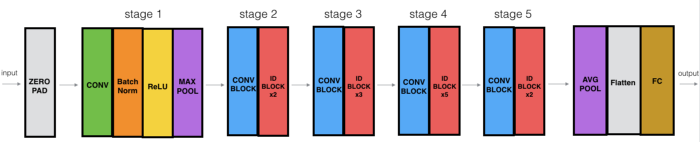
\includegraphics[angle=0, width=1.0\textwidth]{Figures/resnet50.png}
  \caption[ResNet50 architecture overview]{This figure, taken from \citep{Dwivedi:2019:ResNetInKeras}, depicts the original ResNet50 \citep{He:2015:DeepResidualLearningForImageRecognition} architecture composed of five major stages. Each stage contains multiple convolutional layers which results in a very deep-layered architecture.}
  \label{fig:ResNet50Architecture}
  \end{center}
\end{figure}

\noindent The chosen ResNet50 \citep{He:2015:DeepResidualLearningForImageRecognition} model consists of 50 layers, combined in 5 stages, and includes over 23 million trainable parameters. It was one of the very first deep-layered neural networks that introduced a solution to the notorious vanishing gradient problem by its 'skip connection' concept.
\newline\newline
'Skip connection' is done by adding a shortcut from the input to the output of a 'CONV' or 'ID' block, allowing the gradient to flow through. This behaviour, as illustrated in Figure \ref{fig:ResNet50ConvBlock}, makes sure that the subsequent block performs at least as well as the previous. An overview of the composition of all blocks in ResNet50 is presented in Figure \ref{fig:ResNet50Architecture}. 

\begin{figure}[H]
  \begin{center}
  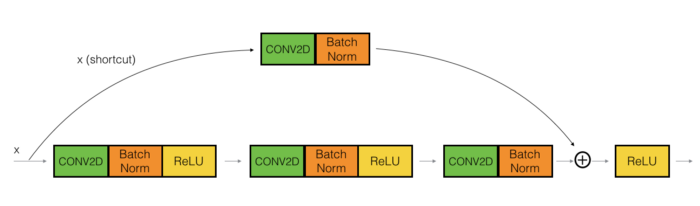
\includegraphics[angle=0, width=0.9\textwidth]{Figures/ResNet50_ConvBlock.png}
  \caption[ResNet50 skip connection]{The figure, taken from \citep{Dwivedi:2019:ResNetInKeras}, depicts the skip connection approach introduced in the ResNet50 \citep{He:2015:DeepResidualLearningForImageRecognition} architecture. Next to adding the original input to the output, a convolution + BatchNorm is performed on the shortcut connection.}
  \label{fig:ResNet50ConvBlock}
  \end{center}
\end{figure}


\subsection{Training} \label{sec:Training&Regularization}
\subsubsection{Pre-trained network}
A pre-trained network is a saved neural network that has previously learned spatial hierarchy of features on a large and general dataset. As recommended by \citet{Chollet:2017:DeepLearningPython} using a pre-trained neural network is a highly effective approach when dealing with a small image dataset. With around 30.000 frames (= 600 video clips), the AFEW-VA dataset \citep{Kossaifi:2017:AFEW-VADatabase} can be considered as such. The utilized VGGFace network was pre-trained on the large-scale face recognition dataset VGGFace2 \citep{Cao:2018:VGGFace2}. This has the advantage, that face recognition poses similar challenges as found in emotion recognition, and by using the pre-trained VGGFace network, already learnt information can be reused for the emotion recognition challenge.

\subsubsection{Fine-tuning}
In order to be able to fine-tune a pre-trained network, it first had to be adapted to the current challenge. Therefore, in this work the classifier got replaced with a Fully-Connected plus two RNN layers. These RNN layers help to capture the tempo-spatial information between frames of a video-clip. The design decision for the classifier was based on previous experiments conducted by \citet{Kollias:2019:AffWild}.
\newline\newline
Due to the random initialization of the custom added classifier, the first step when fine-tuning the model was to train the classifier for a few epochs. At the same time, all other layers from the pre-trained model were not allowed to train and adapt to the new challenge (=frozen). This prevents the error stemming from the random initialization to propagate through the whole network.\citep{Chollet:2017:DeepLearningPython}
\newline\newline
In the second fine-tuning step, the pre-trained neural network was allowed to train and adapt to the new task in accordance with the selected Multi-Phase Fine-Tuning (FT) \citep{Sarhan:2020:MultiPhaseFineTuning} strategy. In contrast to Single-Phase FT where network is trained by unfreezing a set amount of layers at once, in Multi-Phase FT the network is trained by successively unfreezing layers in phases. This is illustrated in Figure \ref{fig:MultiPhaseFT}. In each phase the network's training process is started again, but each time more layers are allowed to be trained and adapted to the new task. As a result, each phase can build on the progress made by the previous phase. According to \citet{Sarhan:2020:MultiPhaseFineTuning} Multi-Phase FT achieves greater accuracy in fewer training epochs in comparison to Single-Phase Fine-Tuning.

\begin{figure}[H]
  \begin{center}
  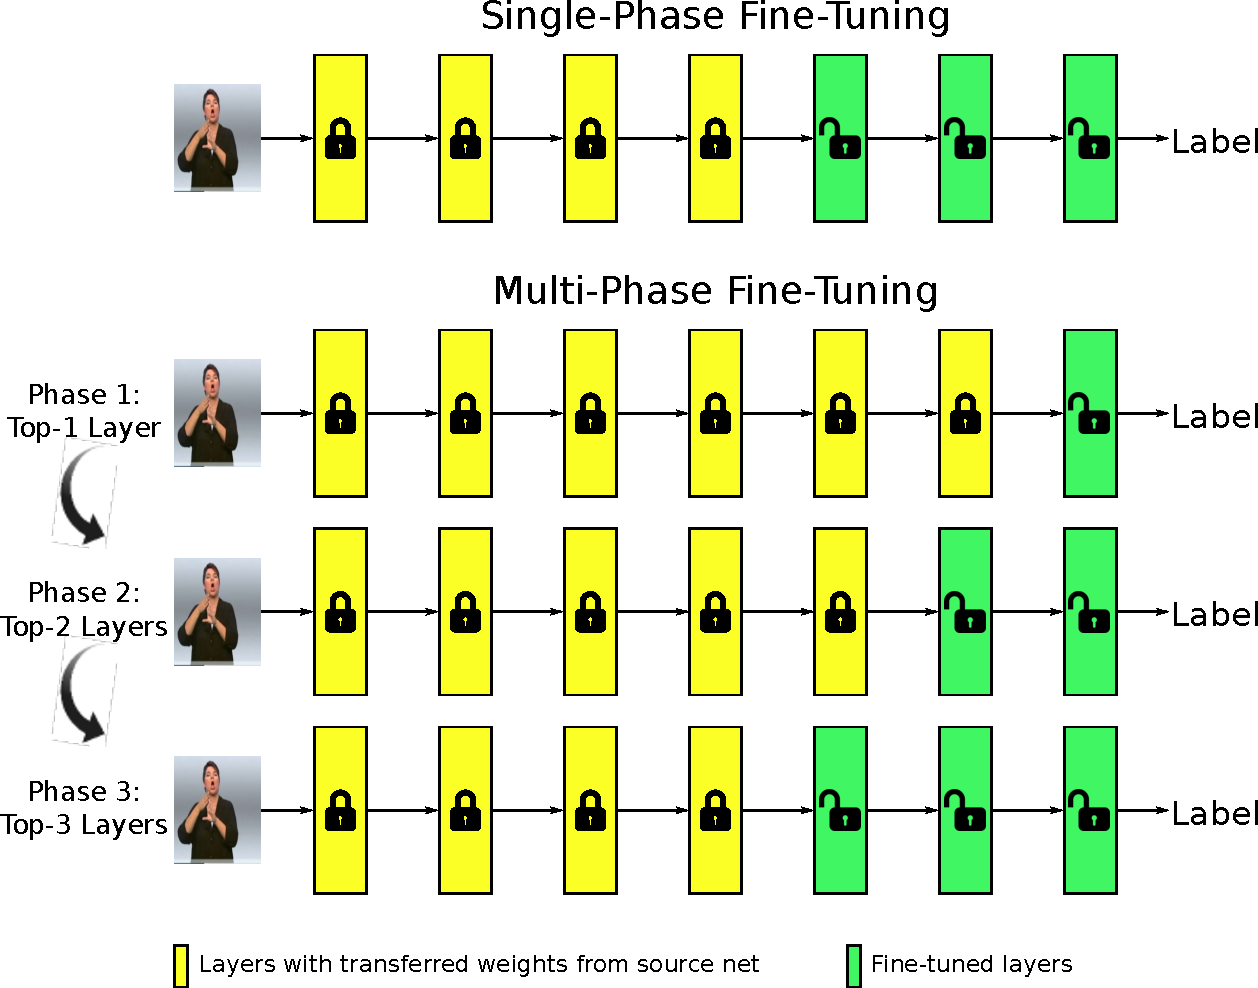
\includegraphics[angle=0, width=0.8\textwidth]{Figures/MultiPhaseFT.pdf}
  \caption[Multi-Phase Fine-Tuning overview]{The image explains the Multi-Phase Fine-Tuning (FT) \citep{Sarhan:2020:MultiPhaseFineTuning} approach. In comparison to Single-Phase FT where layers are unfrozen at once, Multi-Phase FT unfreezes layers in multiple phases. This leads to a greater accuracy in fewer training epochs.}
  \label{fig:MultiPhaseFT}
  \end{center}
\end{figure}

%%%%%%%%%%%%%%%%%%%%%%%%%%%%%%%%%%%%%%%%%%%%%%%%%%%%%%%
\subsection{Regularization}
A central role in developing a successful solution with machine learning is making sure that an algorithm will perform well not only on the training data, but also on previously unseen data. In many machine learning challenges it is common, that a well performing algorithm on the training data performs bad on previously-unseen data. This happens when the model is trying to memorize the training dataset, instead of learning its underlying patterns. This behaviour is called 'overfitting'. Strategies explicitly designed for decreasing overfitting, even at the expense of increasing the training error, are known as regularization. \citep{Goodfellow:2016:DeepLearning}
\newline\newline
An intuitive way to prevent overfitting is to use more training data, as this exposes the model to more data that it needs to find a useful representation for. However, in reality gathering more data is often not a viable option, which is why further regularization techniques are necessary to force the model to focus on the most prominent patterns. The easiest way, according to \citet{Chollet:2017:DeepLearningPython}, is to reduce the neural network's size in terms of trainable parameters. This would result in a reduction of the model's learning capacity.

\subsubsection{Feature removal}
For the here proposed machine learning model it was not possible to increase the amount of training data, as this would make an objective comparison with benchmark paper impossible. Thus, further regularization techniques were applied. The first choice was also to reduce the network's size. The pre-trained VGGFace network already provides a big stack of layers that cannot be removed without losing valuable information. Therefore, the convolution network for the mask, as well as the shared layers at the end of the network were kept at a minimal size.

\subsubsection{Dropout}
Dropout is a very commonly used regularization technique that introduces noise during training by randomly setting a certain percentage of the layer's output values to zero. The Dropout applied in the proposed architecture was determined through extensive experimentation and was applied four times with a rate of 0.5, as illustrated in Figure \ref{fig:MachineLearningModel}. Figure \ref{fig:Dropout} shows an example where a dropout rate of 0.5 was applied to an activation matrix. Applying such a dropout rate allows a network to purposefully forget some information, which makes the learning process harder, but merits a better generalization.

\begin{figure}[H]
  \begin{center}
  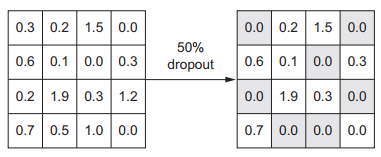
\includegraphics[angle=0, width=0.7\textwidth]{Figures/dropout.PNG}
  \caption[Dropout regularization]{The figure illustrates the application of dropout on a matrix. The applied dropout sets a defined percentage of parameters in an activation matrix to zero \citep{Chollet:2017:DeepLearningPython}. This can increase the generalization ability of a model by increasing the training difficulty.}
  \label{fig:Dropout}
  \end{center}
\end{figure}




\subsubsection{Data Augmentation}

\begin{figure}[htpb]
  \centering
  \subfloat[V: 0.0, A: +0.5]{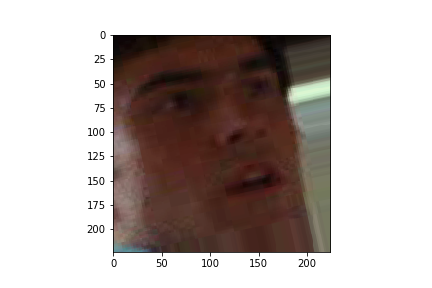
\includegraphics[width=0.5\textwidth]{Figures/001/001_6_00000.png}}
  \hfill
  \subfloat[V: 0.0, A: +0.5]{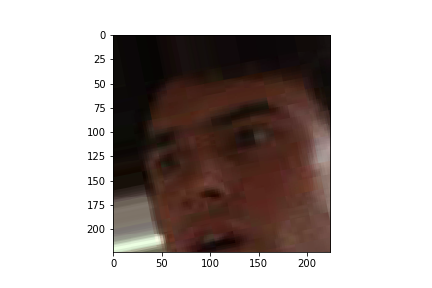
\includegraphics[width=0.5\textwidth]{Figures/001/001_6_00011.png}}
  \hfill
  \subfloat[V: +0.2, A: +0.3]{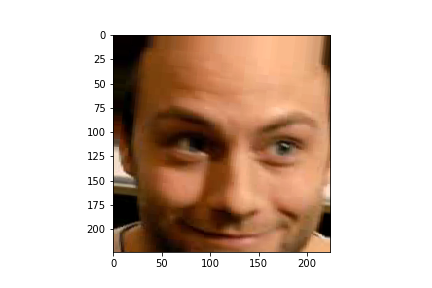
\includegraphics[width=0.5\textwidth]{Figures/002/002_6_00000.png}}
  \hfill
  \subfloat[V: +0.2, A: +0.4]{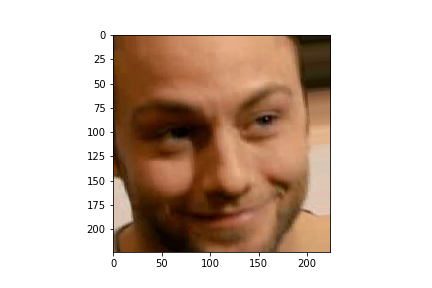
\includegraphics[width=0.5\textwidth]{Figures/002/002_6_00011.png}}
  \hfill
  \subfloat[V: -0.5, A: +0.3]{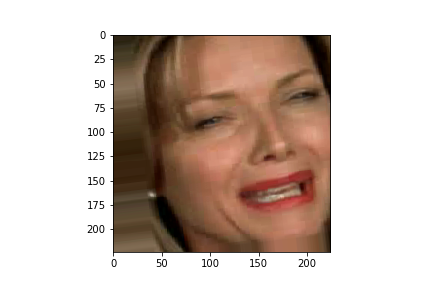
\includegraphics[width=0.5\textwidth]{Figures/576/576_6_00000.png}}
  \hfill
  \subfloat[V: -0.6, A: +0.3]{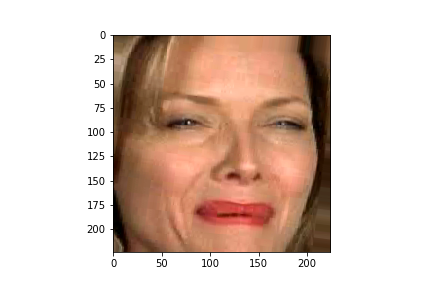
\includegraphics[width=0.5\textwidth]{Figures/576/576_6_00011.png}}
  \caption[Data Augmentation]{These images visualize the augmentation of extracted faces, together with their corresponding labels, expressed by valence (V) and arousal (A) as values ranging from -1 (V: very negative; A: very calming) and +1 (V: very positive; A: very exciting)}
  \label{fig:MethodologyDataAugmentation}
\end{figure}

\noindent Data augmentation is another technique that is used to increase noise during training by randomly transforming existing training samples into slightly different looking images. In that way, the model will see more slightly different images which increases its ability to better generalize from training data. Even though data augmentation was applied during training to both, the face and it's corresponding mask, Figure \ref{fig:MethodologyDataAugmentation} only presents examples from augmented faces.
\newline\newline
The data augmentation applied in the here proposed solution augmented the images randomly with the following parameters:

\begin{itemize}
    \item rotation range from 0 to 15 degrees
    \item width shift range from 0 to 15 percent of the total width
    \item height shift range from 0 to 15 percent of the total height
    \item horizontal flip
    \item brightness shift range from 80 to 120 percent
\end{itemize}

\subsubsection{Hyper-parameter optimization} \label{sec:HyperParameterOptimization}
The ptimization of important hyper-parameters also greatly reduces the effects of overfitting. Two of the most impactful parameters are the learning rate and the batch size.
\newline\newline
An analysis conducted by \citet{Yuanzhi:2019:RegularizationInitialLargeLearningRate} on initial learning rates confirmed that an initially large learning rate can have a regularization effect on the training process. Even though a small initial learning rate might allow for better performance initially, it will not be able to generalize as well as initially large learning rates. The training performed in this Master's thesis made use of an initial learning rate of 0.0001 for the first 3 epochs. Afterwards the training was also started off with a rate of 0.0001, but continuously decreased with each epoch by a factor of 0.95 through a learning rate scheduler.
\newline\newline
Along with the effects of the initial learning rate on improving generalization and reducing the effects of overfitting, \citet{Keskar:2016:LargeBatchTrainingGeneralization} posited that choosing small-batch methods consistently generalize better than large batch methods. Due to memory constraints it was not possible to experiment with large batch sizes, which is why for the here proposed approach a batch size of 2 was chosen. This translates into each batch consisting of two times the sequence length of 45.

%%%%%%%%%%%%%%%%%%%%%%%%%%%%%%%%%%%%%%%%%%%%%%%%%%%%%%%%%

\section{Evaluation \& Metrics}
\subsection{Evaluation} \label{sec:TrainValTestSplit}
Since the AFEW-VA dataset has no official validation and testing set, the AFEW-VA paper proposed by \citet{Kossaifi:2017:AFEW-VADatabase} and the simultaneous VA prediction paper proposed by \citet{Handrich:2020:SimultaneousPredVA} evaluate their models through splitting the AFEW-VA dataset into five disjoint, subject-independent folds. Subsequently, they performed a 5-fold-cross-validation for the prediction of valence and arousal values. 
\newline\newline
Due to time, complexity and resource constraints, it was chosen that this Master's thesis would not use the 5-fold-cross-validation evaluation approach. Instead, it makes use of the more prevalent method for machine learning model evaluation, namely the split of the dataset into a training, validation and test subset. This technique is illustrated in Figure \ref{fig:TrainValTestSplit}. The training and validation subset were used during training to determine the optimal hyper-parameter settings. As these settings influence the performance on the validation subset, a third, independent subset was needed: the testing subset. This subset was used for a final performance evaluation after the optimal hyper-parameters were found.

\begin{figure}[H]
  \begin{center}
  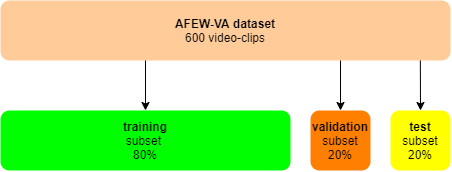
\includegraphics[angle=0, width=0.7\textwidth]{Figures/TrainValTestSplit.png}
  \caption[Dataset training-validation-test split]{The figure shows how the dataset was split into a training, validation and test subset. While training and validation were used for the determination of optimal hyper-parameter settings, the test subset was set aside for a final evaluation of the best performing model.}
  \label{fig:TrainValTestSplit}
  \end{center}
\end{figure}

\subsection{Metrics} \label{sec:Metrics}
Considering the nature of the problem at hand, predicting the values for valence and arousal is better solved through regression, hence a metric such as accuracy, albeit common, will not provide useful information to reflect the performance of the system. Therefore, we stick to the measures used by \citet{Kossaifi:2017:AFEW-VADatabase}, namely root-mean-squared error (RMSE) and Pearson's product-moment correlation coefficient (CORR). 
\newline\newline
RMSE (eq. \ref{eq:RMSE}) is useful in giving the observer a notion of how close the predicted values are to the actual values, while CORR (eq. \ref{eq:CORR}) tells how strong the relationship between the prediction and the actual label is \citep{Chai:2014:RMSE} \citep{Kirch:2008:PearsonCorrelation}.
  
  
\begin{equation} \label{eq:RMSE}
RMSE = \sqrt{(\frac{1}{n})\sum_{i=1}^{n}(y_{i} - x_{i})^{2}}
\end{equation}
\newline\newline
\begin{equation} \label{eq:CORR}
CORR = \frac{{}\sum_{i=1}^{n} (x_i - \overline{x})(y_i - \overline{y})}
{\sqrt{\sum_{i=1}^{n} (x_i - \overline{x})^2(y_i - \overline{y})^2}}
\end{equation}

where
\begin{conditions*}
 x_i  &  the actual ground truth value\\
 y_i  &  the predicted output value \\
 \overline{x}  &  the mean of all ground truth values \\
 \overline{y}  &  the mean of all predicted output values
\end{conditions*}

The RMSE is additionally used as the loss function for the optimization during training.

\subsection{Observation}
In order to find optimal hyper-parameter settings during training, the aforementioned metrics were continuously observed through an early stopping callback, as well as a model checkpoint callback. These callbacks made sure that the last best model, in terms of validation loss, was automatically backed up and that training was stopped as soon as the model successively failed to improve. The callbacks for this work are clearly defined in Figure \ref{fig:EarlyStopping} and \ref{fig:ModelCheckpoint}.\newline

\begin{figure}[H]
  \begin{center}
  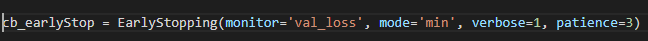
\includegraphics[angle=0, width=0.8\textwidth]{Figures/EarlyStopping.PNG}
  \caption[EarlyStopping callback]{The figure depicts the definition of the early stopping callback, which stops the training process as soon as there has not been any learning progress after a set period of epochs.}
  \label{fig:EarlyStopping}
  \end{center}
\end{figure}

\begin{figure}[H]
  \begin{center}
  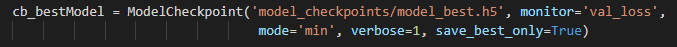
\includegraphics[angle=0, width=0.8\textwidth]{Figures/ModelCheckpoint.PNG}
  \caption[Model checkpoint callback]{The figure shows the definition of the model checkpoint callback, that tracks and automatically saves the weights of the model for the best performing training epoch.}
  \label{fig:ModelCheckpoint}
  \end{center}
\end{figure}

\noindent In essence, these callbacks reduce overfitting by stopping the learning process when no improvement on validation data was detected. Additionally, they allow to objectively compare different hyperparameter-settings of a model's architecture with one another.
\newline\newline
To sum it up, this chapter covered important underlying concepts/techniques for the training and evaluation success of the machine learning model on the AFEW-VA dataset. It is important to point out the combination of the pre-trained VGGFace network with Multi-Phase fine-tuning which facilitated a fast convergence of the training process.